\section{AFL}

\begin{frame}{AFL}{Présentation}
\end{frame}

\begin{frame}{AFL}{Algorithme génétique}
  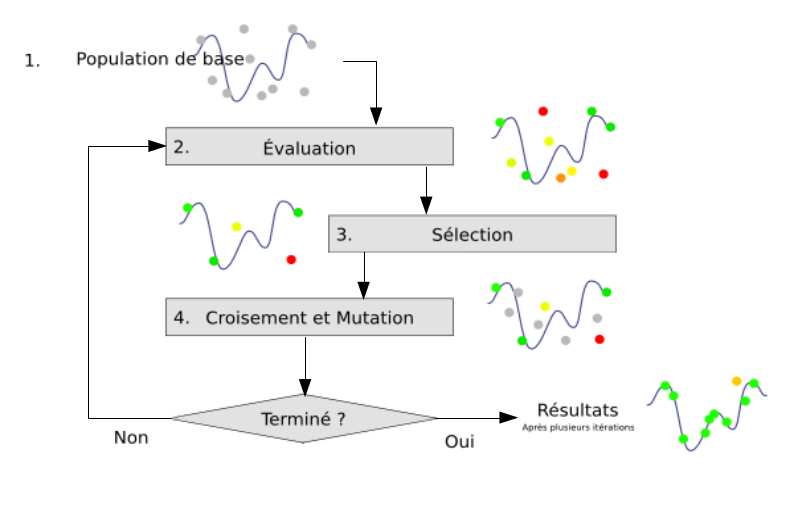
\includegraphics[width=\textwidth]{../medias/schema_genetique.png}
\end{frame}

\begin{frame}{AFL}{Instrumentation}
\end{frame}

\begin{frame}{AFL}{Modèle "fork server" (1)}
  \begin{columns}[t]
    \begin{column}{0.49\textwidth}
      \begin{block}{"classique"}
        \begin{itemize}
        \item \lstinline{execve()}
          \begin{itemize}
          \item copie du programme en mémoire
          \item \lstinline{ld-linux.so} charge les librairies partagées
          \end{itemize}
        \item \lstinline{waitpid()}
        \item tout recommencer avec une autre entrée
        \end{itemize}
        \vspace{3.5ex}
      \end{block}
    \end{column}

    \begin{column}{0.49\textwidth}
      \begin{block}{"fork server"}
        \begin{itemize}
        \item \lstinline{execve()} "classique"
        \item programme cible instrumenté
          \begin{itemize}
          \item "pause" avant le \lstinline{main} du programme
          \item \lstinline{fork()} pour copier le processus
          \item \lstinline{waitpid()} pour surveiller les enfants
          \end{itemize}
        \item communication entre alf-fuzz et programme parent avec un \lstinline{pipe}
        \end{itemize}
      \end{block}
    \end{column}
  \end{columns}
\end{frame}

\begin{frame}{AFL}{Modèle "fork server" (2)}
  \begin{columns}[t]
    \begin{column}{0.5\textwidth}
      \begin{center}
        \textbf{"classique"}
      \end{center}

      \bigskip
      \begin{figure}
        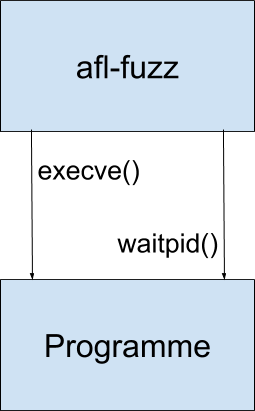
\includegraphics[width=.4\textwidth]{../medias/classique.png}
      \end{figure}
    \end{column}

    \begin{column}{0.5\textwidth}
      \begin{center}
        \textbf{"fork server"}
      \end{center}

      \begin{figure}
        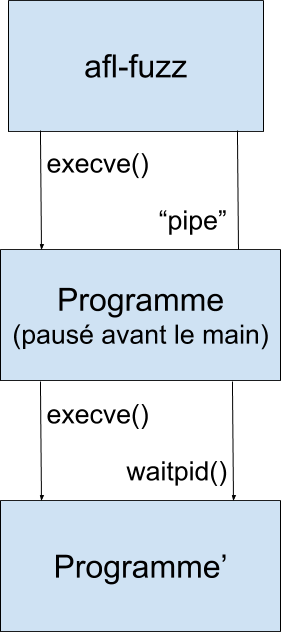
\includegraphics[width=.4\textwidth]{../medias/fork-server.png}
      \end{figure}
    \end{column}
  \end{columns}
\end{frame}
